\documentclass{article}
\usepackage{tikz}

\begin{document}

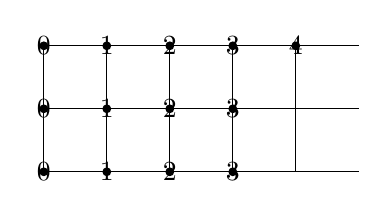
\begin{tikzpicture}[scale=0.8]
    % Draw horizontal lines
    \draw (0,0) -- (5,0);
    \draw (0,-1) -- (5,-1);
    \draw (0,-2) -- (5,-2);

    % Draw dots and labels
    \foreach \x in {0,...,4} {
        \fill (\x,0) circle (2pt);
        \node at (\x,0) {\x};
    }
    \foreach \y in {0,...,3} {
        \fill (\y,-1) circle (2pt);
        \node at (\y,-1) {\y};
    }
    \foreach \z in {0,...,3} {
        \fill (\z,-2) circle (2pt);
        \node at (\z,-2) {\z};
    }

    % Connect points with lines
    \draw (0,0) -- (0,-1);
    \draw (0,-1) -- (0,-2);
    \draw (1,0) -- (1,-1);
    \draw (1,-1) -- (1,-2);
    \draw (2,0) -- (2,-1);
    \draw (2,-1) -- (2,-2);
    \draw (3,0) -- (3,-1);
    \draw (3,-1) -- (3,-2);
    \draw (4,0) -- (4,-1);
    \draw (4,-1) -- (4,-2);
\end{tikzpicture}

\end{document}